% Figure 5: original qualitative grid with no sensor/column headings.
% Sensor identities, column order, and per-frame MAE are explained in the caption.
% Experimental image pixels and vector error values are unchanged.
\begin{tikzpicture}[x=1bp,y=1bp]
\useasboundingbox (0,0) rectangle (271.4,92);
\node[anchor=south west,inner sep=0pt] at (0,1) {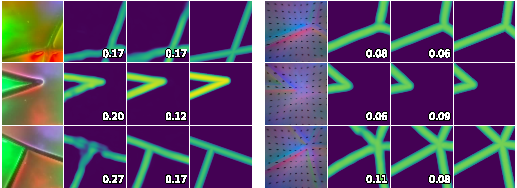
\includegraphics[width=248.4bp,height=90bp]{figures/qualitative_assets/image_grid.pdf}};
% Lossless rotation of the original color bar: low (purple) at bottom, high (yellow) at top.
\node[anchor=south west,inner sep=0pt] at (252.3,5) {
\includegraphics[width=3bp,height=80.4bp]{figures/qualitative_assets/depth_colorbar_vertical.png}};
\definecolor{QualDepthMax}{rgb}{0.993248,0.906157,0.143936}
\definecolor{QualLegendEdge}{gray}{0.40}
% Preserve the original upper-limit extension.
\fill[QualDepthMax] (252.3,85.4) -- (253.8,89.42) -- (255.3,85.4) -- cycle;
\draw[QualLegendEdge,line width=0.28bp] (252.3,5) -- (252.3,85.4) -- (253.8,89.42) -- (255.3,85.4) -- (255.3,5) -- cycle;
\foreach \y/\tick in {5/0.0,31.8/0.4,58.6/0.8,85.4/1.2}{%
  \draw[QualLegendEdge,line width=0.28bp] (255.3,\y) -- (256.5,\y);
  \node[anchor=west,inner sep=0pt,font=\fontsize{5.2bp}{6bp}\selectfont] at (257.5,\y) {\tick};
}
\node[rotate=90,inner sep=0pt,font=\fontsize{5.2bp}{6bp}\selectfont] at (268.0,45.2) {Depth [mm]};
\end{tikzpicture}%
